%%%%%%%%%%%%%%%%%%%%%%%%%%%%%%%%%%%%%%%%%%%%%%%%%%%%%%%%%%%%%%%%%%%%%%%%%%%%%%%%
%                              Document Settings                               %
%%%%%%%%%%%%%%%%%%%%%%%%%%%%%%%%%%%%%%%%%%%%%%%%%%%%%%%%%%%%%%%%%%%%%%%%%%%%%%%%

\documentclass[a4paper,12pt]{article}
\usepackage[utf8]{inputenc}
%%%%%%%%%%%%%%%%%%%%%%%%%%%%%%%%%%%%%%%%%%%%%%%%%%%%%%%%%%%%%%%%%%%%%%%%%%%%%%%%
%                                   Margins                                    %
%%%%%%%%%%%%%%%%%%%%%%%%%%%%%%%%%%%%%%%%%%%%%%%%%%%%%%%%%%%%%%%%%%%%%%%%%%%%%%%%

\addtolength{\oddsidemargin}{-1.cm}
\addtolength{\textwidth}{2cm}
\addtolength{\topmargin}{-2cm}
\addtolength{\textheight}{3.5cm}

%%%%%%%%%%%%%%%%%%%%%%%%%%%%%%%%%%%%%%%%%%%%%%%%%%%%%%%%%%%%%%%%%%%%%%%%%%%%%%%%
%                                   Packages                                   %
%%%%%%%%%%%%%%%%%%%%%%%%%%%%%%%%%%%%%%%%%%%%%%%%%%%%%%%%%%%%%%%%%%%%%%%%%%%%%%%%

\usepackage[pdftex]{graphicx}	% Include graphics
\usepackage{float}				% Place floats inline, use the [H] placement
\usepackage{array}				% Additional tables features


%%%%%%%%%%%%%%%%%%%%%%%%%%%%%%%%%%%%%%%%%%%%%%%%%%%%%%%%%%%%%%%%%%%%%%%%%%%%%%%%
%                                   Document                                   %
%%%%%%%%%%%%%%%%%%%%%%%%%%%%%%%%%%%%%%%%%%%%%%%%%%%%%%%%%%%%%%%%%%%%%%%%%%%%%%%%

\begin{document}
	
	% Title page
	% Title page
	\begin{titlepage}
		\begin{center}
			
			% University Logo
			
\includegraphics[width=0.6\textwidth]{../images/up_logo.jpg}\\[2.0cm] 
			
			
			\textsc{\LARGE CS@UP Time Series Prediction}\\[1.0cm]
			
			
			\textsc{\Large System Requirements Specification Document}\\[0.75cm]
			
			
			\textsc{\Large COS301 - Capstone Project}\\[0.75cm]
			
			
			% Students/Contributors Table
			\textbf{\huge \\ Team:}
			\huge NewGen Leaders \\
			\begin{flushright} \large
				Claudio Da Silva		\emph{u14205892} \newline
				Dedr\'e Olwage	    	\emph{u15015239} \newline
				Merrisa Joubert			\emph{u15062440} \newline
				Murray Le Roux	    	\emph{u15311644} \newline
			\end{flushright}
			\small Department of Computer Science, University of Pretoria \\ 
			
			
		\end{center}
		
		% Report Declaration		
		\noindent By submitting this document we confirm that we have read and are aware of the University of Pretoria's policy on academic dishonesty and plagiarism and we declare that the work submitted in this assignment is our own as delimited by the mentioned policies. We explicitly declare that no parts of this assignment have been copied from current or previous students' work or any other sources (including the internet), whether copyrighted or not. We understand that we will be subjected to disciplinary actions should it be found that the work we submit here does not comply with the said policies.
		
		\begin{center}
			
			% Fill page
			\vfill
			
			% Date
			{\large \today}
			
		\end{center}
		
	\end{titlepage}
    
    \tableofcontents
    % An overview of the SRS document
    \section{Introduction}
    	
        % Specify the purpose of this SRS and the intended audience
        \subsection{Purpose}
        
        % Identify product by name, explain what the product will and will not do, describe the uses of the product including objectives, goals and benefits
The purpose of this document is to present a detailed description of the Time Series Prediction System. It will explain the purpose and features of the system, the interfaces of the system, what the system will do, the constraints under which it must operate and how the system will react to external stimuli. This document is intended for both the stakeholders and the developers of the system.
        \subsection{Scope}
The system will be used to enter, view, and edit student marks. It will include a prediction system that will use the student marks to make predictions on the outcomes of the students results at the end of the semester. These predictions will be used by lecturers to identify students who need extra help to pass the semester. The predictions may also be used to identify whether the teaching strategies of the lecturer are working as well as they expected it to. The system will allow students to view their marks and it will include an element of gamification that aims to improve student motivation. The ultimate goal of the system is to improve student results. The system also aims to improve the manner in which teaching assistants, tutors and lecturers record marks.
        \subsection{Definitions,Acronyms and Abbreviations}
        \begin{center}
\begin{tabular}{ |c|c| } 
\hline
Term & Definition \\
\hline
Stakeholder & A person, whom is not a developer, that has an interest in the product\\
\hline
Time series prediction & A number of algorithms that use current input data to predict future data\\
\hline
\end{tabular}
\end{center}
        \subsection{References}
        % Outline the rest of the SRS and how it is organized 
        This document defines the overall Description of the product. It then explains the product perspective and gives details about the different interfaces of the system. The document further explains the functions and characteristics of the system. System constraints and requirements are elaborated.
        
    \pagebreak
    % Provide an overview of the product
    
    \section{Overall Description}
    
    	% Describe the context of the product and its relations and interfaces to other components of the total system. Block diagrams may be used to show the context and relationships. Describe also the characteristics and limits on primary and secondary memory, modes of operation, backup and recovery, and site specific requirements.
    	\subsection{Product perspective}
    	
        	\subsubsection{System Interfaces}
        	
        	A system interface defines the interface between a sub-system and the system as a whole.\\\\ 
        	
        	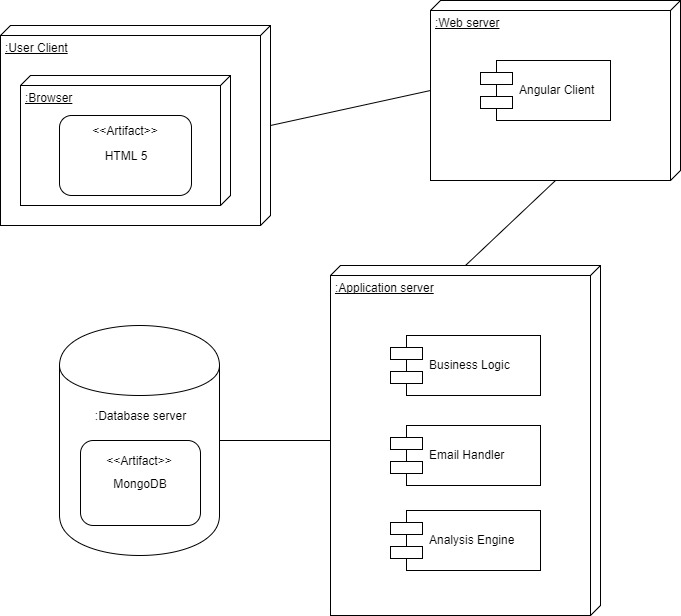
\includegraphics[width=0.9\textwidth]{../diagrams/system_overview.jpg}
        
        	\begin{itemize}
        		\item \textbf{Client side}
	        	\begin{itemize}
	        		\item The client will receive requests from the user via a method called REST calls. The client then interfaces with the server side by passing along those calls, and receiving the responses, with which it can process as needed.
	        	\end{itemize}
        	\end{itemize}
        
        	\begin{itemize}
	        	\item \textbf{Server side}
	        	\begin{itemize}
	        		\item The server will receive requests from the client in the form of a REST call. The server will process this, and respond as necessary. The server will also interface with the local mail client, as well as the data analysis engine, as a separate running entity on the server host. The server is also required to interface with the database instance of MongoDB assigned to it within the configuration.
	        	\end{itemize}
        	\end{itemize}
        	
            \subsubsection{User Interfaces}
            
            There are currently only two ways to interface with the system:
           	
           	\begin{itemize}
            	\item \textbf{The web client}
            	\begin{itemize}
            		\item Users will be able to access the software through an intuitive Web
            		Interface, and hence through any device that has an HTML 5 compliant browser with javascript enabled.
            	\end{itemize}
            \end{itemize}
        
        	\begin{itemize}
        		\item \textbf{The command console}
        		\begin{itemize}
        			\item Users will be able to access certain features via the terminal, whether it is to run or configure the program. The only constraint is this can only be done on the device on which the software is running, or via access to it such as telnet.
        		\end{itemize}
        	\end{itemize}
            
            \subsubsection{Hardware Interfaces}
            
             	\begin{itemize}
            	\item \textbf{User side}
            	\begin{itemize}
            		\item The user will require a physical device upon which a browser can be run (Computer, phone, tablet etc.)
            	\end{itemize}
            \end{itemize}
            
            \begin{itemize}
            	\item \textbf{Client side}
            	\begin{itemize}
            		\item The client will require a physical or cloud device on which to run.
            		\item The client will require an active Internet connection to be maintained (Ethernet or WIFI access)
            	\end{itemize}
            \end{itemize}
            
            \begin{itemize}
            	\item \textbf{Server side}
            	\begin{itemize}
            		\item The server will require a physical or cloud device on which to run.
            		\item The server will require an active Internet connection to be maintained (Ethernet or WIFI access)
            	\end{itemize}
            \end{itemize}
            
            \subsubsection{Software Interfaces}
            
           	\begin{itemize}
            	\item \textbf{User side}
            	\begin{itemize}
            		\item Users will require a browser with which to access the software
            	\end{itemize}
            \end{itemize}
        
	        \begin{itemize}
	        	\item \textbf{Client side}
	        	\begin{itemize}
	        		\item The client software will require an OS upon which to run. The software is multi-platform so any will do.
	        		\item The client will require NodeJS 6 or higher upon which to run.
	        		\item The client will require the Angular CLI be installed as a global dependency.
	        	\end{itemize}
	        \end{itemize}
        
        	\begin{itemize}
        		\item \textbf{Server side}
        		\begin{itemize}
        			\item The server software will require an OS upon which to run. The software us multi-platform so any will do.
        			\item The server will require NodeJS 6 or higher upon which to run.
        			\item The server will require a connection to a running instance of MongoDB
        		\end{itemize}
        	\end{itemize}
            
            \subsubsection{Communication Interface}
            
           	\begin{itemize}
            	\item \textbf{User side}
            	\begin{itemize}
            		\item Users will connect to the client via the web using an HTTP/HTTPS protocol on either port 80 or 443.
            	\end{itemize}
            \end{itemize}
            
            \begin{itemize}
            	\item \textbf{Client side}
            	\begin{itemize}
            		\item The client will provide communication via the web, exposed either via port 80 or port 443.
            		\item The client will communicate with the server via a process called REST calls, using JSON payloads.
            	\end{itemize}
            \end{itemize}
            
            \begin{itemize}
            	\item \textbf{Server side}
            	\begin{itemize}
           			\item The server will provide communication via the web, exposed either via port 80 or port 443.
	            	\item The client will communicate with the server via a process called REST calls, using JSON payloads.
	            	\item The server will communicate with MongoDB via a specified port, configured within the server's configuration file.
	            	\item The server will communicate sending email, using a SMTP protocol either via port 25 or 587.
            	\end{itemize}
            \end{itemize}
            
            \subsubsection{Memory}
            
            Most information regarding the system will reside in a central
            MongoDB database, including but not limited to:
            
            \begin{itemize}
            	\item User information
            	\item Module data
            \end{itemize}
        	The size recommended will depend on the amount of data you plan to store.\\\\
           	Logs are also to be stored, in the form of text files, and will be backed up on a regular basis, thus will require enough free space to stay available A minimal of 1GB is recommended.\\\\	
           	Another thing to be stored is objects. These include things such as PDFs. Links will be used to access them, and them may be stored either locally, or in another location as desired.\\\\
           	Clustering will make an attempt to use up all available RAM and CPU usage where possible to increase performance, unless stated otherwise. A minimal of at least 500mbs RAM is recommended.
            
            \subsubsection{Operations}
            
              
            \begin{itemize}
            	\item \textbf{Client side}
            	\begin{itemize}
            		\item Client operations will focus around addition and retrieval of marks and the information surrounding it. No prior knowledge should be needed before using this system, and thus it should be intuitive. The only required knowledge should be that of the spreadsheet formats to use.
            	\end{itemize}
            \end{itemize}
        
        	  
        	\begin{itemize}
        		\item \textbf{Client side}
        		\begin{itemize}
        			\item Server operations around processing the requests sent from the client. No/minimal maintenance should be needed in order to keep operations running. The system administrator should be able to maintain and manage the server with minimal knowledge of the system intricacies, meaning it should be intuitive as far as possible. Operations should be configurable as much as possible via the configurations file. 
        		\end{itemize}
        	\end{itemize}
        
            Backup and recovery operations should be defined in the case of software failure. 
            
            \subsection{Site Adaptation Requirements}
            
            The system should be adaptable to a changing university environment. A change in the way things are done should be simple to fix, such as a new staff hierarchy or the way marks may be calculated. It should preferably also not be dependent on any part of a single university, and should instead easily adapt into any educational institution that follows the same patterns.\\\\            
            The design of the system should be able to adapt to whatever device is required, as it is expected to be functional on multiple devices. 
            
        \subsection{Product Functions}
        
        The functions of the product fall into 2 main categories:
        
        	\begin{itemize}
        		\item \textbf{Marks management}
        		\begin{itemize}
        			\item Simply put, the system needs to create a simple and intuitive way for users, dependent on their permissions, to manipulate marks, either by adding new ones, or viewing them. This requires other functions such as management of users and their permissions, and also the ability to add the assignments and modules that the marks themselves belong to.
        		\end{itemize}
        	\end{itemize}
        
        	
        	\begin{itemize}
        		\item \textbf{Marks and student analysis}
        		\begin{itemize}
        			\item The core functionality of the system is the analysis of marks and the notification of problem areas. Simply put the system needs to be able to, based on a users history of marks over time, determine their risk of failure and level of help required, and notify the relevant parties as soon as possible. The aspect of gamification also falls under this category, as students are to be motivated by these results if possible.
        		\end{itemize}
        	\end{itemize}
        
        \pagebreak
        
        \subsection{User Characteristics}
        
       	Users are people with ties to the university, who are stakeholders in some part to the addition and retrieval of marks. The initial idea in order to create a more decoupled system, is to grant users different permissions based on a list of permissions the application has defined. This creates no pre-defined user types, other than the superuser with all permissions and the standard user with none. There are two types of permissions:
        \begin{itemize}
        	\item \textbf{Global}
        	\begin{itemize}
        		\item This is a permission set for the entirety of the application. If set, this grants access whenever that permission is requested, anywhere in the application, regardless of module division. Some permissions only have a global version, such as the permission to create users.
        	\end{itemize}
        	\item \textbf{Local}
        	\begin{itemize}
        		\item This is a permission set for only a specific module of the program. If set, this grants access whenever that permission is requested, but only in modules to which that permission is set as true. In all other modules that permission will be denied.
        	\end{itemize}
        \end{itemize}
        By default, the initial user is created as a "Superuser", where all permissions for the program are set to true. This superuser can then from there create or import further users and set their permissions accordingly. By default, any new user created is automatically set to have no permissions at all, thus the standard user.\\\\
        
        % Describe the restrictions on the solution space or options of the developer
        \subsection{Constraints}
        
        \begin{itemize}
       		\item \textbf{Hardware constraints}
        	\begin{center}
        		
        		\begin{tabular}{ |c|c| }
        			
        			\hline
        			Constraint Number & Constraint Description \\
        			\hline
        			C1 & An active connection must consistently be maintained \\
        			\hline
        			
        		\end{tabular}
        	\end{center}
        	\item \textbf{Software constraints}
               \begin{center}
               	
		        	\begin{tabular}{ |c|c| }
		        		 
		        		\hline
		        		Constraint Number & Constraint Description \\
		        		\hline
		        		C1 & Marks spreadsheets must be in a specified format \\
		        		\hline
		        		C2 & User data must be in a specified format to import  \\
		        		\hline
		        		C3 & Only links to objects may be stored ( e.g assignment PDFs) \\
		        		\hline
		        		C4 & Browsers used must be HTML 5 compliant and have JavaScript active \\
		        		\hline
		        		
		        	\end{tabular}
        		\end{center}
        \end{itemize}
    
    	\pagebreak
    	
        %List the factors that affect the requirements
        \subsection{Assumptions and Dependencies}
        A number of factors that may affect the requirements specified in the SRS include:
        \begin{itemize}
        	\item It is assumed that there is an existing standard for marksheets and that all staff will follow this standard to ensure efficient processing of the marks.
        	\item It is assumed that there is a hierarchy structure of staff in place, and permissions will follow in that order. 
        	\item It is assumed that users will be part of the university system, and in order to use this software, they must be a part of this system.
        	\item It is assumed that users will have Internet access at all times when trying to use this system, thus it will offer no offline capabilities.
        	
        \end{itemize}
    
    	\pagebreak
    	    	
    	\section{Specific Requirements}
    
    	\subsection{External Interface Requirements}
    	
    	It may be possible that the system will be required to interface with Fitchfork, an external marking tool at the university of Pretoria, in order to easily obtain marks and deliver them.\\\\	
    	The system should be able to interface with the mail server currently in place at the institution, or any other kind of cloud based service.
    	
        \subsection{Functional Requirements}
        	\subsubsection{Business Requirements}
        	\begin{itemize}
        	\item The system is initialized with a single Dean as the main Admin with all rights
        	\item The Dean adds HODs to the system
        	\item HODS can then add lecturers, and assistant lecturers to the system
        	\item Lecturers add teaching assistant, tutors, and students to their specific modules
        	\item Students write tests and complete practicals and assignments
        	\item The results of the tests, practicals and assignments are entered into the system by tutors, assistant lecturers and lecturers
        	\item The system performs time series prediction on these results and sends reports about the results and predictions to the lecturer
        	\item The lecturer may then choose to contact students who need extra help
        	\end{itemize}
        	\subsubsection{Security Requirements}
        	\begin{itemize}
        	\item The system will limit access to authorized users
        	\item Roles are assigned to user. Each role will have its own abilities. Roles include: student, teaching assistant, tutor, assistant lecturer, lecturer, head of department, and Dean.
        	\item Students can only view and query marks
        	\item Teaching assistants may add marks, but these marks have to be reviewed by a lecturer or assistant lecturer to be submitted to the database
        	\item Assistant Lecturers and lecturers may modify, view, and add or remove marks
        	\item The Dean has to add HODs to the system, HODS will add Lecturers, Lecturers will add assistant lecturers and assistant lecturers will add teaching assistants and tutors to the system
        	\end{itemize}
        	
        \subsection{Performance Requirements}
        \begin{itemize}
        \item The system will be required to work with potentially thousands of students.
        \item The system will manage many simultaneous notifications
        \item The system will need to manage the simultaneous login of a multitude of users.
        \end{itemize}
        
        \subsection{Design Constraints}
        \begin{itemize}
        \item Time limit
        \item The application will be web based and must be cross-platform
        \end{itemize}
        
        \subsection{Software System Attributes}
        	\subsubsection{Accessibility}
        	
        	\subsubsection{Accuracy}
        	\subsubsection{Administrability}
        	\subsubsection{Compatibility}
        	\subsubsection{Integrity}
        	\subsubsection{Maintainability}
        	\subsubsection{Mobility}
        	\subsubsection{Traceability}
        	\subsubsection{Vulnerability}
        	\subsubsection{Usability}
        \subsection{Other Requirements}
        \begin{itemize}
        \item Gamification elements are required to improve student motivation
        \item Anonymous leader boards will be displayed to all students
        \end{itemize}
    \section{Appendixes}
    
    \section{Index}
    
    \pagebreak  

\end{document}
